\documentclass{beamer}
\usepackage{tikz}
% Define Color
\definecolor{rose}{rgb}{1.0, 0.0, 0.56}
% Defined Commands
\newcommand{\mycomment}[1]{}
\newcommand{\lattice}{\mathcal{L}}
\newcommand{\blue}{\textcolor{blue}}
\newcommand{\red}{\textcolor{red}}
\newcommand{\green}{\textcolor{green}}
\newcommand{\rose}{\textcolor{rose}}
%\newcommand{\doublecheckb}{\blue{\checkmark\kern-0.55em\checkmark}}
%\newcommand{\doublecheckr}{\red{\checkmark\kern-0.55em\checkmark}}
\begin{document}
\begin{frame}
\begin{center}
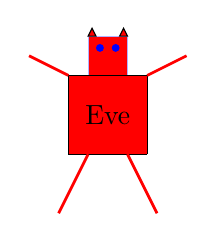
\begin{tikzpicture}[scale = 0.5]



	\fill [red] (0,0) rectangle (2,2) ;
	\node at (1,1) {Eve};
	%\fill [blue!30] (1,3) circle [radius = 1];
	\draw [blue!30, fill= red] (0.5,2) rectangle (1.5,3);
	\draw[step=2cm, thin,fill = red] (0,0) grid (2,2);
	\draw [line width =1, red] (0.5,0) -- (-0.25,-1.5);
	\draw [line width =1, red] (1.5,0) -- (2.25,-1.5);
	\draw [line width =1, red] (0,2) -- (-1,2.5);
	\draw [line width =1, red] (2,2) -- (3,2.5);
	\fill [blue] (0.8,2.7) circle [radius = 0.1];
	\fill [blue] (1.2,2.7) circle [radius = 0.1];
	\draw[fill=red] (1.3,3) -- (1.5,3) -- (1.4,3.2) -- cycle;
	\draw[fill=red] (0.5,3) -- (0.7,3) -- (0.6,3.2) -- cycle;

\end{tikzpicture}
\end{center}
\end{frame}
\end{document}